% !TEX root = scientific-computing.tex
%
\hypertarget{ch:functional-programming}{%
\chapter{Functional Programming and an Introduction to
Writing fast
code}\label{ch:functional-programming}}

This chapter introduces ideas of
\href{https://en.wikipedia.org/wiki/Functional_programming}{functional
programming}, which is a way to think about programming using functions.
Typically this requires a language that falls into the category of a
\emph{functional computer language}, one of which is Julia. In short, a
language that has this feature has a function (or procedure) as a
fundamental element of the language and one of which can be passed as
arguments.

\section{Functional vs. Non-functional forms}

Often functional programming is used with arrays or lists of other data.  Let 
\begin{jlblock}[fp]
arr=collect(1:5)
\end{jlblock}

Here's a simple example of taking all of the elements of \texttt{arr} and finding another array which is the square of each number. In a statement-based point-of-view:

\begin{jlblock}[fp]
newarr=zeros(5)  # this an array of zeros of length 5
for i=1:5
  newarr[i]=arr[i]^2
end
newarr
\end{jlblock}
%
which returns the array \jlc[fp]{print(map(i->i^2,[1,2,3,4,5]))} \printpythontex[verb].

From a functional point-of-view, a common method is a \texttt{map} command which takes in an array and produces another array in which a function acts on each element of the array. In this case, the function is the square.
%
\begin{jlblock}[fp]
f(x)=x^2
arr=[1,2,3,4,5]
map(f,arr)
\end{jlblock}
%
or more simply using an \textbf{anonymous function},
%
\begin{jlblock}[fp]
map(x->x^2,arr)
\end{jlblock}

The key to this example is the ability to pass the function as an argument to the \texttt{map} command. Once you get a feeling for functional programming, it is often an easier way to write code.\footnote{An extreme example of this is to avoid using any for loops after understanding maps and other related functions.  Although, often this can happen, it doesn't 1) make the underlying code any faster or 2) any easier to understand, so I don't generally prescribe to this philosophy.}

\subsection{Anonymous Functions}

The example above included in the first argument \verb!x->x^2!, which is an example of a \emph{anonymous function}.  In short, it is anonymous because we didn't assign it to a name and instead just applied the function to the \verb|map| command.  

Any time that a function is used in the form \verb!->!, it is anonymous.  For example, if we want to sum the contents of the array \jlb[fp]{A=[1,2,3,4,5]}, one way is to 
\begin{jlblock}[fp]
reduce((x,y)-> x+y, A)
\end{jlblock}
which results in \jlc[fp]{print(reduce( (x,y)->x+y,A))} \printpythontex[verb], the sum of the elements of the array.  We'll see the \verb!reduce! function in the next section.  Concentrate right now on the \verb!(x,y)->x+y!, an anonymous functions can take on more than one variable.  


\subsection{Exercise}

\begin{itemize}
\item Write a statement-based loop to take the array \texttt{{[}1,2,3,4,5{]}} and output an array that is the reciprocal of each number.
\item Write a functional-based code using the \texttt{map} command to do the same.
\end{itemize}

\section{Reducing an array}\label{sect:reduce:array}

The \texttt{map} command in general takes in an array and returns an array. Another common task with arrays is to  reduce the entire array to a single value. If \jlb{arr=[1,2,3,4,5]}, then we can sum the values with the \texttt{reduce} command as in:
%
\begin{jlblock}[fp]
reduce((x,y)->x+y,arr)
\end{jlblock}
%
which returns \jlc{print(reduce(+,arr))}\printpythontex[verb]. 

To multiply all numbers, we can type:
%
\begin{jlblock}[fp]
reduce((x,y)->x*y,arr)
\end{jlblock}
and the result is \jlc[fp]{print(reduce(*,arr))}\printpythontex[verb].  In both of these cases, there is a little bit hidden, so let's look at these in more detail. 
\begin{enumerate}
\item  First, the first argument of the \texttt{reduce} command is a 2-argument (or binary) function.  
\item Secondly, the operation is done on all numbers on the array, but needs to start with some value (because it is a binary function).  In the sum case, the initial value is 0 (by default) and in the multiply case it is 1.  
\end{enumerate}


These are perhaps obvious examples and each of these have the built-in functions \texttt{sum} and \texttt{prod} that find the sum and product of an array. 

Let's look at an example that returns the number of array elements that are greater than zero:
%
\begin{jlblock}[fp]
numPos(arr) = reduce((n,val) -> val > 0 ? n+1 : n, arr, init=0)
\end{jlblock}
%
and then if it is tested on an array of both positive and negative
numbers:
%
\begin{jlblock}[fp]
numPos([-3,5,8,-2,11])
\end{jlblock}
%
this returns \jlc[fp]{print(numPos([-3,5,8,-2,11]))}\printpythontex[verb]. How this works is as follows. There are two values
associated within reduce from the function. The first is \texttt{n} and the second is \texttt{val}.

\begin{enumerate}
\item  the variable \texttt{n} is initially 0 (this is the \texttt{init=0}
  part of the function call)
\item  On the first step, \texttt{val} takes on the first value in the array
  (or \texttt{-3}). It is checked if it is positive and if so, return
  \texttt{n+1} or \texttt{n}.  Since n=0 and \texttt{-3} is not positive, then the function returns 0.
\item  On the second step, \texttt{val} is 5 and this time the function
  returns \texttt{n+1} or 1
\item  \texttt{val} is 8 and the function returns \texttt{n+1} or 2
\item  \texttt{val} is -2 and the function returns \texttt{n} or 2
\item  \texttt{val} is 11 and the function returns \texttt{n+1} or 3.
\item  Since the array has been passed through, the result is the last value or 3.
\end{enumerate}

\subsection{Exercise}

\begin{itemize}
\item Write a reduce function that will count the number of times the string
``hi'' appears in an array. Test it on \jlv[fp]{["hi","bye","hi","hello"]} and other arrays of strings.  

\item What does \jlb[fp]{reduce(string,["J","u","l","i","a"],init="")} do?
\end{itemize}

\hypertarget{the-mapreduce-function}{%
\section{\texorpdfstring{The \texttt{mapreduce}
function}{The mapreduce function}}\label{the-mapreduce-function}}

The
\href{http://docs.julialang.org/en/release-0.5/stdlib/collections/\#Base.mapreduce}{\texttt{mapreduce}} function is perhaps more helpful than \texttt{reduce}. For example, if we want to sum the squares of each number in an array, then \texttt{mapreduce} can do this easily.

\begin{jlblock}
mapreduce(x->x^2,+,[1,2,3],init=0)
\end{jlblock}
%
is a short-hand way to do $1^2+2^2+3^2=14$. Note: julia also has a version of the \texttt{sum} function that can apply a function.  For example, 
%
\begin{jlblock}[fp]
sum(x->x^2,[1,2,3])
\end{jlblock}
also returns \jlc{print(sum(x->x^2,[1,2,3]))}\printpythontex[verb]. 

\subsection{Exercise}

In calculus, an important infinite series is 
%
\begin{align*}
1 + \frac{1}{4} + \frac{1}{9} + \frac{1}{16} + \cdots
\end{align*}
and although we can't sum an infinite number of terms, a finite version of this is still useful.  

Use \texttt{mapreduce} to sum the first 20 terms.  Hint: use \jlb[fp]{arr=collect(1:20)}. 

\section{Mapping a Function over an 2D array}

Above, we saw the \verb!map! function which applies a function over each element of the array.  We will see in Chapter \ref{ch:prob-models} that the \verb!mapslices! functions is quite helpful. 

Consider the array \jlb[fp]{A=[i+j for i=1:10,j=1:3]} which returns
\jlc[array]{display(A)} \printpythontex[verbatim]
 
If we want to sum down the columns of the array, we can enter 
\begin{jlblock}[fp]
mapslices(sum,A,dims=[1])
\end{jlblock}
which returns \jlc[fp]{print(mapslices(sum,A,dims=[1]))} \printpythontex[verb], which is a 1D array with the column sums.  The \verb!mapslices! function needs three arguments, a function that can take an array, a 2D array and the keyword \texttt{dims} which says how to apply the sum.  Note: we can also replace the command \verb!sum! with \verb!+! as well.   

If instead we wanted to sum along rows, then 
\begin{jlblock}[fp]
mapslices(sum,A,dims=[2])
\end{jlblock}
which returns \jlc[fp]{display(mapslices(sum,A,dims=[2]))} \printpythontex[verbatim] which is a column vector. Although note that this is a 2D array.  The function \texttt{mapslices} always returns an array of the same number of dimensions as the original.  

\subsection{Exercises}

Using the matrix \jlb[fp]{A=[i+j for i=1:10,j=1:3]}, 
\begin{itemize}
\item evaluate \jlb[fp]{mapslices(prod,A,dims=[1])}.  What does that function do?
\item evaluate \jlb[fp]{mapslices(prod,A,dims=[2])}.  What does that function do?
\item use the \verb!mapslices! function to find the maximum element in each row.  
\item use the \verb!mapslices! function to find the maximum element in each column.  
\end{itemize}




\section{Writing fast code}

The last part of this chapter will show one aspect of writing fast code, an important aspect of scientific computing. We will study a number of ways to sum up the first $n$ counting numbers and determine why the timing of
things are different. Also, we are going to test the various types of integers as well to determine the speed of things with that. In each case we are going to create a function and then time it. 

\begin{description}
\item[Attempt \#1]

Let's start by making an array of all of the numbers, then summing them
in a for loop:

\begin{jlblock}[fastcode]
function sum1(n::Int)
  local arr = collect(1:n)
  local sum = 0
  for i in arr
    sum += i
  end
  sum
end
\end{jlblock}

 On a relatively slow machine:
%
\begin{jlverbatim}
@time sum1(1_000_000)
\end{jlverbatim}
%
returns
%
\jlc[fastcode]{display(@time sum1(1_000_000))} \printpythontex[verbatim].

The \texttt{@time} is called a macro, which is similar to a function, however is more flexible.  In this case, it calculates the time it takes, number of allocations and memory allocated.  The macro then returns the value of the function 

If we repeat this for the sum of the first billion counting numbers: 
%
\begin{jlverbatim}
@time sum1(1_000_000_000)
\end{jlverbatim}
%
%
it takes a while:\jlc[fastcode]{display(@time sum1(1_000_000_000))} \printpythontex[verbatim].

The big difference between these is the total memory allocation. There is a 1000-fold increase in memory allocated (note the MiB or megabytes versus GiB or gigabytes).  This also shows about a 2000-fold increase in time.  

Allocating memory is a time-expensive endeavor.  Also, even though the machine that I ran this on has 16 gigabytes, perhaps it couldn't get all 7.5 GiB it needed for this operation at once.  This is shown with the 0.05\% gc time, which mean garbage collection.  In short, there was some time needed to handling so much memory. 

If you have some patience, try this will 2 billion or more and see the results.  You will probably need more allocation time and should be at least twice as long.  

\item[Attempt \#2:] The big difference seemed to be the total memory allocation, so let's
try a version where we don't allocate the array.

\begin{jlblock}[fastcode]
function sum2(n::Integer)
    local sum = 0
    for i=1:n
        sum+=i
    end
    sum
end
\end{jlblock}

and running it as \jlv[fastcode]{@time sum2(1_000_000_000)} we get:
%
\jlc[fastcode]{display(@time sum2(1_000_000_000))} \printpythontex[verbatim]
%
and notice that the time has shrunk to zero--we'll see later why this is true. If we try for larger numbers, such as \jlv{@time sum2(100_000_000_000))}, we get:
%%
%
\begin{jlcode}[fastcode]
display(@time sum2(100_000_000_000))
\end{jlcode}
and results in \printpythontex[verbatim]
which still takes almost no time, but notice that that the result is not correct.  Why?  Consider the ideas from Chapter \ref{ch:data-types}.  


\item[Attempt \#3:]

Hopefully you thought about the strange result above.  If you thought overflow, give yourself a gold star.  To avoid this, let's write a \texttt{BigInt} version of this:
%
\begin{jlblock}[fastcode]
function sum3(n::Int)
    local sum = big(0)
    for i=1:n
        sum+=i
    end
    sum
end
\end{jlblock}
%
and:
%
\begin{jlblock}[fastcode]
@time sum3(1_000_000)
\end{jlblock}
%
returns \jlc[fastcode]{display(@time sum3(1_000_000))} \printpythontex[verbatim]

Comparing this with the results at the beginning of Attempt \#1, shows that BigInts are much slower as mentioned in Chapter \ref{ch:data-types}.  

\begin{jlblock}[fastcode]
@time sum3(10_000_000)
\end{jlblock}
%
returns \jlc[fastcode]{display(@time sum3(10_000_000))} \printpythontex[verbatim]
%
which is about 10 times slower, so it appears that this is linear as possibly as expected. This isn't practical to find much larger sums though. 

\item[Attempt \#4:]

Let's trying using the \texttt{reduce} function on BigInts:

\begin{jlblock}[fastcode]
function sum4(n::Int)
    reduce(+,1:big(n))
end
\end{jlblock}

Then:
%
\begin{jlblock}[fastcode]
@time sum4(1_000_000)
\end{jlblock}
%
returns: \jlc[fastcode]{display(@time sum4(1_000_000))} \printpythontex[verbatim]
%
Notice that this allocates about 91 MiB of memory, which isn't a lot, but this is probably due to the \texttt{BigInt} allocations.  Also, this is about twice the amount of time as that in Attempt \#3. Notice also a significant amount of gc (garbage collection) time.  

 Also,
%
\begin{jlblock}[fastcode]
@time sum4(10_000_000)
\end{jlblock}
%
returns: \jlc[fastcode]{display(@time sum4(10_000_000))} \printpythontex[verbatim]
%
which is about 10 times slower that the previous one, and still 1.6 times the speed of \texttt{sum3} for the same number \texttt{n}. 

\item[Attempt \#5:]

Let's use the built-in \texttt{sum} command. Entering:

\begin{jlblock}[fastcode]
@time sum(1:big(10)^6)
\end{jlblock}

returns \jlc[fastcode]{@time sum(1:big(10)^6)}\printpythontex[verabtim]
%
and note that higher powers of 10 do not increase the time much. For example,

\begin{jlblock}[fastcode]
@time sum(1:big(10)^20)
\end{jlblock}
%
results in \jlc[fastcode]{display(@time sum(1:big(10)^20))}\printpythontex[verbatim]
 What is going on? How is this so fast?  Think about this and we'll answer it below. 

\end{description}

\subsection{Exercise}

Repeat Attempts \#1--\#4 for \texttt{Int128}.  That is, make sure that the calculations are being done using this type.  For the \texttt{for} loops, start with 
\begin{jlverbatim}[fastcode]
local sum = Int128(0)
\end{jlverbatim}
and for the \texttt{reduce} function use \jlv[fastcode]{Int128(n)} instead of \jlv[fastcode]{big(n)}.

Compare your results with those above.  

\section{Summary of Results}

There were a lot of factors going on in the above example.  Here's a summary.

\begin{itemize}
\item \emph{Allocating an array is expensive (in terms of memory and time).}  In Attempt \#1, we created an array using the \texttt{collect} function. The creation was why this took so much time. 
\item \emph{BigInts and \texttt{Int128} are slower than \texttt{Int64}s.}   We noticed that switching from \texttt{Int64} to \texttt{BigInt} in Attempt \#2 to \#3, there was a significant drop in speed.  In short, \texttt{BigInt}s are slow.  Only use them when needed.  

You should have noticed from the exercise that \texttt{Int128} is a viable alternative to \texttt{Int64} if you need larger integers.  \texttt{Int128} is slower than \texttt{Int64}, but still much better than \texttt{BigInt}.  Only use \texttt{BigInt} when you need really large integers. 

\item \emph{Sometimes julia is super smart about some operations.}  In both Attempt \#2 and Attempt \#5, we got much shorter times than expected.  In both, you would expect summing 1000 times more numbers would take 1000 times longer, but this isn't true.  In both cases, julia recognizes that integers are begin summed and is probably using the formula
\begin{align*}
1+2+3 + \cdots + n & = \frac{n(n+1)}{2}
\end{align*}
and using this formula can be done for any number $n$ with no summing at all. 
\end{itemize}

\section{Computing Fibonacci Numbers} \label{sect:faster:fibonacci}

In section \ref{sect:recursion}, there was an exercise to use recursion to find the fibonacci numbers.  A possible solution to this is:
\begin{jlblock}[fibonacci]
fibonacci(n::Integer) = (n==1 || n==2) ? 1 : fibonacci(n-1) + fibonacci(n-2)
\end{jlblock}
where we have used the ternary \texttt{if-then-else}.  Note: if \texttt{n} is 1 or 2, then 1 is returned, if not it uses the recursive formula.  The first 10 fibonacci numbers are found with
\begin{jlblock}[fibonacci]
map(fibonacci,1:10)
\end{jlblock}
and this results in \jlc[fibonacci]{print(map(fibonacci,1:10))} \printpythontex[verb].

It is fast to find the fibonacci numbers for smaller values, but consider
\begin{jlblock}[fibonacci]
@time fibonacci(40)
\end{jlblock}
results in \jlc[fibonacci]{display(@time fibonacci(40))} \printpythontex[verbatim]
%
and if we find \jlv{@time fibonacci(41)}, it is about twice as long.   To consider what happens, let's look at \jlv{fibonacci(5)}.  Inside the function, it calls \jlv{fibonacci(4)} and \jlv{fibonacci(3)}.  Each of these then called the previous two.  This can be seen in the following tree graph where $f(n)$ is the fibonacci function:
\begin{center}
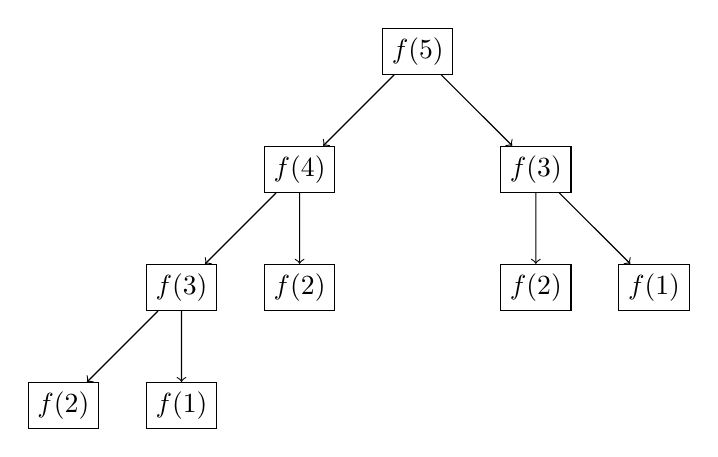
\begin{tikzpicture}[scale=0.75]
\node (A) at (0,10) [draw] {$f(5)$};
\node (B) at (-2,8) [draw] {$f(4)$};
\node (C) at (2,8) [draw] {$f(3)$}; 
\draw[->] (A) -- (B);
\draw[->] (A) -- (C); 

\node (D) at (-4,6) [draw] {$f(3)$};
\node (E) at (-2,6) [draw] {$f(2)$};
\draw[->] (B) -- (D);
\draw[->] (B) -- (E);

\node (F) at (2,6) [draw] {$f(2)$}; 
\node (G) at (4,6) [draw] {$f(1)$}; 
\draw[->] (C) -- (F);
\draw[->] (C) -- (G);

\node (H) at (-6,4) [draw] {$f(2)$};
\node (I) at (-4,4) [draw] {$f(1)$};  
\draw[->] (D) -- (H);
\draw[->] (D) -- (I); 
\end{tikzpicture}
\end{center}

Since each of the endpoints (either $f(2)$ or $f(1)$ requires and evaluation as does each arrow, there are a total of 13 evaluations for this.  If we define:
%
\begin{jlblock}[fibonacci]
function fibonacciEval(n::Integer)
  global num_evals
  if n==1 || n==2 
    num_evals +=1 
    return 1
  else
    num_evals += 2
    return fibonacciEval(n-1) + fibonacciEval(n-2)
  end
end
\end{jlblock}
then 
\begin{jlblock}[fibonacci]
num_evals=0
fibonacciEval(5)
num_evals
\end{jlblock}
returns \jlc[fibonacci]{print(num_evals)} \printpythontex[verb]. Also
\begin{jlblock}[fibonacci]
num_evals=0
fibonacciEval(20)
num_evals
\end{jlblock}
returns \jlc[fibonacci]{print(num_evals)} \printpythontex[verb]~and
\begin{jlblock}[fibonacci]
num_evals=0
fibonacciEval(21)
num_evals
\end{jlblock}
returns \jlc[fibonacci]{print(num_evals)} \printpythontex[verb]~ and notice that finding the 21st fibonacci number takes about 60\% more operations and therefore would take about this much longer.  

Thinking about this result shows that we aren't doing things efficiently.  If we have already calculated the 19th and 20th fibonacci numbers, why does it take an extra 60\% longer?  Basically this is because we aren't saving the results to be reused. 

\subsection{A still-recursive, but much faster version of Fibonacci} 

As we saw above, the standard recursive version of \verb!fibonacci! function is very slow.\footnote{in fact, it is $O(e^n)$ {\color{red} REALLY?} as we will see.}
We now attempt to find a faster version. Instead of calculating every previous fibonacci number, we will use an array and if the value is already calculated, just look it up in the array or if not, calculate it recursively.  Consider
\begin{jlblock}[fibonacci]
function fibonacci2(n::Integer)
  numbers = zeros(Int64,n)  # need an array of length n
  numbers[1:2] .= 1         # the first two fibonacci numbers are 1
  function fib(k::Integer)
    if numbers[k] > 0
      return numbers[k]  # if we know the number just return it
    end
    numbers[k-1] = fib(k-1)  # these two lines call fib recursively, but 
    numbers[k-2] = fib(k-2)  # if the value is known return it
    numbers[k] = numbers[k-1] + numbers[k-2]  # still the same definition.
  end
  fib(n)
end
\end{jlblock}
%
and try finding fibonacci numbers with this instead.  In fact, \jlb[fibonacci]{@time fibonacci2(100)} returns
\begin{jlcode}[fibonacci]
print(@time fibonacci2(100))
\end{jlcode}
\printpythontex[verbatim]
%
whis is a fraction of the time it took to do the 40th fibonacci number with the original function. The exercise below explores the \verb!fibonacci2! function.   

Note that in the \verb!fibonacci2! function, we use arrays to store all of the fibonacci numbers.  We will see arrays in Chapter \ref{ch:arrays}, but the point of this example is to show that 1) recursion is often a very nice and compact way to write a function, and 2) can be highly inefficient.  We realized that we were never reusing the numbers that were being computed and the best way to store these were in an array. 

Also, you probably noticed that we had a function called \verb!fib! inside the \verb!fibonacci2! function.  We did this because \verb!fib! used the array created in \verb!fibonacci2!.  There were other ways to do this, but this is a very nice example of a function within a function.

\subsection{Exercise}

\begin{enumerate}
\item Determine which fibonacci number results in an overflow for \texttt{Int64}. Do this by trial and error with the \verb!fibonacci2! function.   
\item Rewrite the \verb!fibonacci2! function to return a \verb!BigInt! version if $n$ is greater than or equal to the number in \#1.  
\item Find the first 200 fibonacci numbers. 
\end{enumerate}




